\documentclass[twocolumn,a4paper,11pt]{scrartcl}

% Language and font encoding
\usepackage[spanish,es-noshorthands]{babel}
\usepackage[utf8]{inputenc}
\usepackage[T1]{fontenc}

% Other necessary packages
\usepackage{graphicx}
\usepackage{amsmath}
\usepackage{cite}

% Title information
\title{Óptica Física}
\author{Brian David Leiva. ECFM-USAC}
\date{Febrero, 2025}

\begin{document}

\maketitle

\begin{abstract}
En esta práctica estudiamos experimentalmente los fenómenos de difracción e interferencia de la luz. Se utilizó un montaje óptico que incluía un láser He-Ne, lentes para expandir el haz, y una lente condensadora para proyectar los patrones en una pantalla. Se observaron y midieron los patrones de difracción de Fraunhofer producidos por un agujero circular y los patrones de interferencia generados por una doble rendija. Las posiciones de los máximos en ambos patrones se midieron y compararon con las predicciones teóricas. Los resultados mostraron una buena concordancia entre los valores experimentales y teóricos, verificando la validez de las expresiones que describen estos fenómenos ópticos. Este trabajo permitió una comprensión práctica de conceptos fundamentales en óptica física y demostró la aplicabilidad de los modelos teóricos en situaciones experimentales reales.
\end{abstract}

\section{Objetivos}
El propósito principal de esta práctica es doble. En primer lugar, se busca obtener experimentalmente el patrón de difracción producido por un agujero pequeño, así como el patrón de interferencia generado por una doble rendija. En segundo lugar, se pretende verificar la validez de las expresiones teóricas que describen la ubicación de los máximos y mínimos en ambos patrones.

\section{Marco teórico}

La difracción de Fraunhofer ocurre cuando un frente de onda plano interactúa con un obstáculo cuyas dimensiones son comparables a la longitud de onda de la luz incidente. Este fenómeno se observa en una pantalla distante, donde la distancia D cumple la condición $D \gg a$, siendo a la dimensión característica del obstáculo.

Para obtener el patrón de difracción de Fraunhofer, utilizamos un arreglo experimental que incluye un láser como fuente de luz, lentes para expandir el haz (L1 y L2), y una lente condensadora (L3) para proyectar el patrón en la pantalla. La posición del n-ésimo máximo de difracción, yn, para ángulos pequeños, está dada por la ecuación \cite{serway}:

\begin{equation}
y_n = \frac{nD\lambda}{a}
\end{equation}

donde λ es la longitud de onda de la luz, D es la distancia a la pantalla, y a es el ancho de la apertura.

Por otro lado, el patrón de interferencia se produce cuando un frente de onda plano interactúa con dos o más obstáculos. En el caso de una doble rendija, cada rendija tiene un ancho a y están separadas por una distancia d. Las posiciones de los máximos (y+n) y mínimos (y-n) de interferencia están dadas por:

\begin{equation}
y^+_n = n\frac{D\lambda}{d}
\end{equation}

\begin{equation}
y^-_n = (n + \frac{1}{2})\frac{D\lambda}{d}
\end{equation}

Para máximos cercanos al centro del eje óptico, la distancia entre ellos es aproximadamente constante:

\begin{equation}
\Delta y = \frac{D\lambda}{d}
\end{equation}

Estas ecuaciones nos permitirán analizar y verificar los resultados experimentales obtenidos en la práctica.

\section{Diseño experimental}

\subsection{Componentes}
Para llevar a cabo este experimento, se utilizaron los siguientes componentes:
\begin{itemize}
    \item Láser He-Ne
    \item Lentes de 5mm, 50mm y 5000mm de distancia focal
    \item Porta objetos
    \item Objeto con patrones de agujeros circulares (LH 469 96)
    \item Objeto con patrones de rendijas dobles (LH 469 92)
    \item Colimador
    \item Diafragma de iris
    \item Pantalla traslúcida
    \item Espejo de primera reflexión
    \item Jinetillos
    \item Rieles Ópticos
\end{itemize}

\subsection{Montaje experimental}
El montaje experimental se realizó siguiendo el esquema mostrado en la Figura \ref{fig:montaje}. Los componentes se dispusieron sobre rieles ópticos en el siguiente orden: láser, lente de 5mm, lente de 50mm, diafragma, obstáculo (agujero circular o doble rendija), lente de 5000mm y pantalla.

\begin{figure}[h]
    \centering
    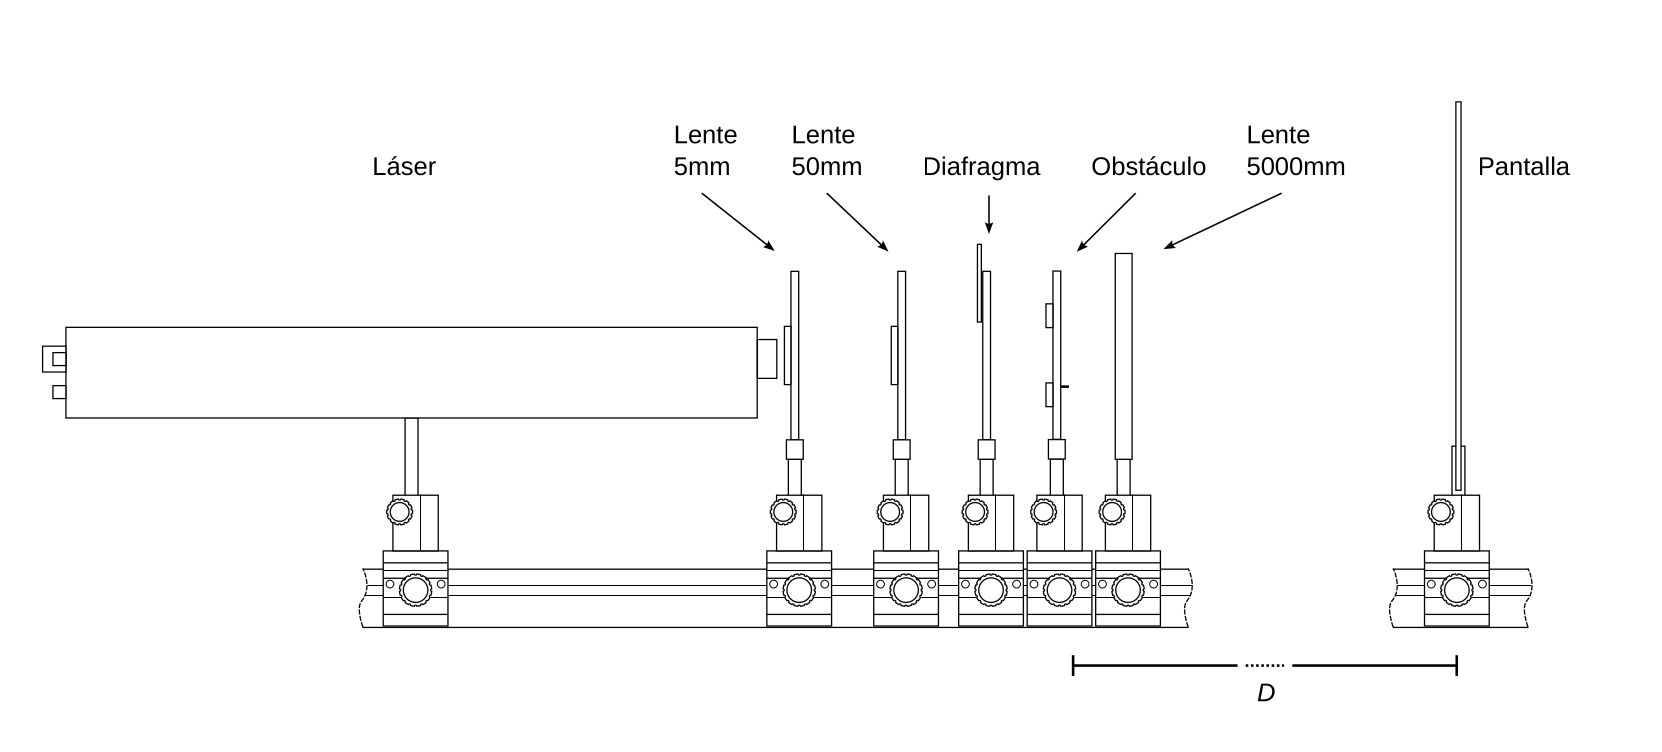
\includegraphics[width=0.6\textwidth]{montaje_experimental_2.png}
    \caption{Esquema del montaje experimental}
    \label{fig:montaje}
\end{figure}

\subsection{Procedimiento}
El procedimiento experimental se llevó a cabo siguiendo estos pasos:

\begin{enumerate}
    \item Se colocaron el láser, el diafragma y la pantalla sobre el riel óptico, asegurando una distancia de aproximadamente 5000 mm entre la lente condensadora y la pantalla.
    
    \item Se verificó la alineación de los elementos, asegurando que el haz del láser pasara por el centro del diafragma e incidiera en el centro de la pantalla.
    
    \item Se montaron las lentes en el siguiente orden:
    \begin{itemize}
        \item Lente de 5000mm
        \item Lente de 50mm
        \item Lente de 5mm
    \end{itemize}
    Se ajustó la distancia entre las lentes de 5mm y 50mm para obtener un punto intenso y definido en la pantalla.
    
    \item Para el experimento de difracción, se colocó el objeto con agujeros circulares en el porta objetos, haciendo incidir el haz del láser sobre el agujero con diámetro mayor.
    
    \item Se midieron las distancias donde aparecían los máximos en el patrón de difracción circular.
    
    \item Para el experimento de interferencia, se sustituyó el objeto por el patrón de rendija doble, haciendo incidir el haz sobre la doble rendija más pequeña.
    
    \item Se midieron las distancias donde aparecían los máximos en el patrón de interferencia.
\end{enumerate}

En ambos casos, se utilizó el colimador para evitar que la luz del láser incidiera sobre otros agujeros o rendijas no deseados.

\section{Resultados y discusión}

\subsection{Patrón de difracción de Fraunhofer}

En este experimento, se observó el patrón de difracción de Fraunhofer producido por un agujero circular. La distancia entre el obstáculo y la pantalla de observación fue de D = 5.00 ± 0.01 m. Esta gran distancia asegura que estamos en el régimen de Fraunhofer, donde se cumple la condición $D \gg a$, siendo $a$ el diámetro del agujero.

La Figura \ref{fig:diffraction_pattern} muestra el patrón de difracción observado en la pantalla.

\begin{figure}[h]
    \centering
    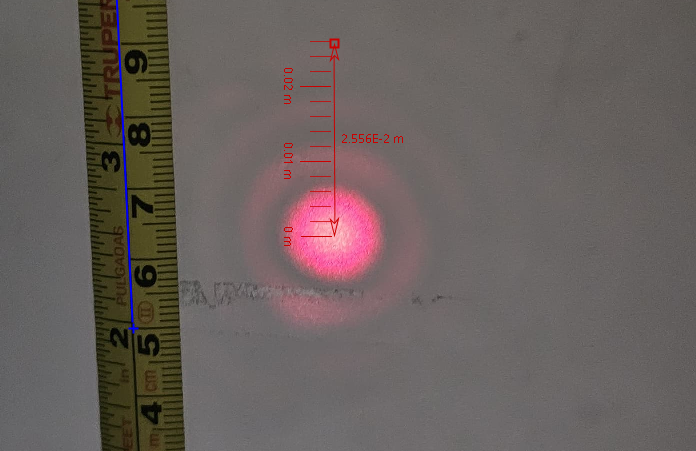
\includegraphics[width=0.4\textwidth]{fraunhoffer.png}
    \caption{Patrón de difracción de Fraunhofer observado para un agujero circular}
    \label{fig:diffraction_pattern}
\end{figure}

Se midieron las distancias desde el centro del patrón hasta los máximos de difracción. La Tabla \ref{tab:diffraction_maxima} presenta estos datos:

\vspace{1em}
\begin{table}[h!]
    \centering
    \begin{tabular}{|c|c|c|}
        \hline
        n & $y_m$ (mm) & $y_t$ (mm) \\
        \hline
        1 & 6.43 ± 1 & 6.59 \\
        2 & 12.68 ± 1 & 13.18 \\
        3 & 19.19 ± 1 & 19.78 \\
        4 & 25.56 ± 1 & 26.37 \\
        \hline
    \end{tabular}
    \caption{Distancias medidas ($y_m$) y teóricas ($y_t$) a los máximos de difracción}
    \label{tab:diffraction_maxima}
\end{table}
\vspace{1em}

Estos datos experimentales nos permiten verificar la validez de la ecuación teórica para la posición de los máximos de difracción:

\begin{equation}
y_n = \frac{nD\lambda}{a}
\end{equation}

donde $y_n$ es la distancia del n-ésimo máximo al centro del patrón, $D= 5000 mm $ es la distancia a la pantalla, $\lambda = 632.81646 nm $ es la longitud de onda del láser, y $a = 0.12 mm$ es el diámetro del agujero.

Observamos que las distancias medidas aumentan linealmente con el orden del máximo, lo cual es consistente con la predicción teórica. 
% \end{table}

\subsection{Patrón de interferencia de doble rendija}

Para el experimento de doble rendija, se utilizó una separación entre rendijas de d = 0.6 mm. La Figura \ref{fig:interference_pattern} muestra el patrón de interferencia observado en la pantalla.

\begin{figure}[h]
    \centering
    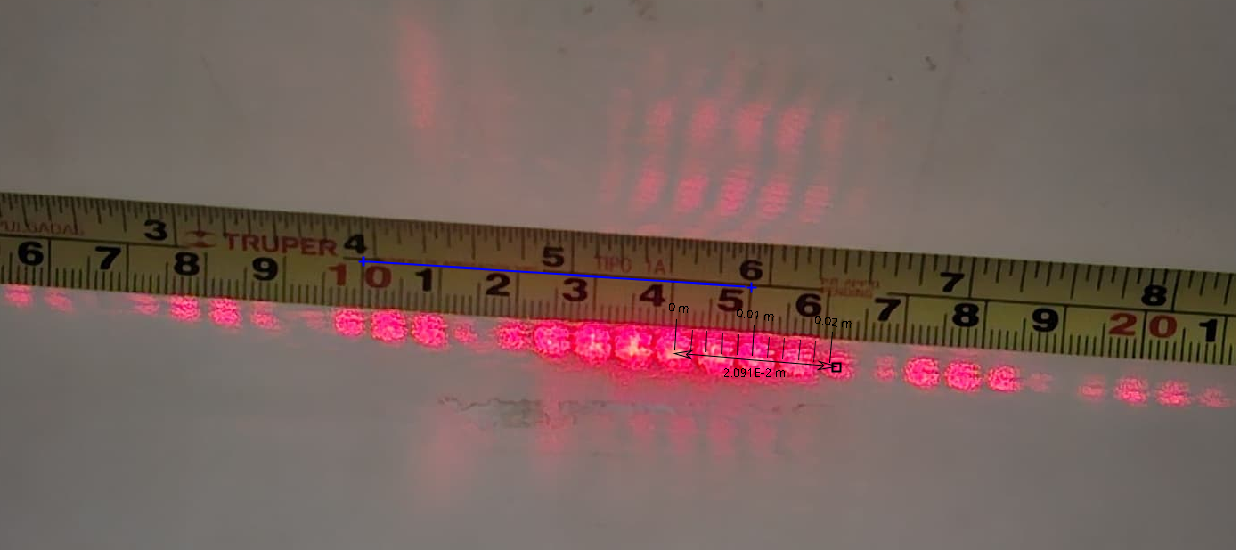
\includegraphics[width=0.4\textwidth]{double_slit.png}
    \caption{Patrón de interferencia observado para una doble rendija}
    \label{fig:interference_pattern}
\end{figure}

Se midieron las distancias desde el centro del patrón hasta los máximos de interferencia. La Tabla \ref{tab:interference_maxima} presenta estos datos, donde n es el orden del máximo:

\vspace{1em}
\begin{table}[h!]
    \centering
    \begin{tabular}{|c|c|c|}
        \hline
        n & $y_m$ (mm) & $y_t$ (mm) \\
        \hline
        1 & 5.30 ± 0.1 & 5.27 \\
        2 & 9.75 ± 0.1 & 10.55 \\
        3 & 15.71 ± 0.1 & 15.82 \\
        4 & 20.91 ± 0.1 & 21.09 \\
        \hline
    \end{tabular}
    \caption{Distancias medidas ($y_m$) y teóricas ($y_t$) a los máximos de interferencia para doble rendija}
    \label{tab:interference_maxima}
\end{table}
\vspace{1em}

Estos datos experimentales nos permiten verificar la validez de la ecuación teórica para la posición de los máximos de interferencia:

\begin{equation}
y_n = n\frac{D\lambda}{d}
\end{equation}

donde $y_n$ es la distancia del n-ésimo máximo al centro del patrón, $n$ es el orden del máximo, $D$ es la distancia a la pantalla, $\lambda$ es la longitud de onda del láser, y $d$ es la separación entre las rendijas.

\section{Conclusiones}

1. Se lograron obtener experimentalmente los patrones de difracción de Fraunhofer para un agujero circular y de interferencia para una doble rendija.

2. Las expresiones teóricas para la ubicación de los máximos en ambos patrones fueron verificadas satisfactoriamente. Las posiciones medidas se ajustaron bien a la ecuación teórica.

3. El montaje experimental demostró ser efectivo para la observación clara de los patrones de difracción e interferencia, permitiendo mediciones precisas.


\bibliographystyle{ieeetr}
\bibliography{referencias}  % Asegúrate de crear un archivo referencias.bib con tus referencias

\end{document}